\documentclass[a4paper,12pt]{article}

% Use ISO date format
\usepackage[english, iso]{isodate}

% Make everything look a little better
\usepackage{microtype}

% Author, year refrencing
\usepackage{natbib}

\usepackage{fancybox}
\usepackage{boxedminipage}

\usepackage{setspace}
\onehalfspacing

\usepackage{color}

% Proper table lines
\usepackage{booktabs}
% More space above tables for caption
\setlength{\abovetopsep}{0.1em}

% typeset chemistry
\usepackage{chemformula}

% Change page size
\usepackage[inner=0.4in, outer=0.3in, twoside, tmargin=0.3in, bmargin=0.5in]{geometry}

% Change caption formatting
\usepackage[hang, bf]{caption}

% Unit typesetting
\usepackage{siunitx}

% plotting
\usepackage{pgfplots}

% import graphics
\usepackage{graphicx}
  \DeclareGraphicsExtensions{.jpg, .pdf, .mps, .png}
  \graphicspath{{graph/}}

% Put bibliography in table of contents, and change name to "References"
\usepackage[nottoc,numbib]{tocbibind}
\settocbibname{References}

% Change punctuation for references
\bibpunct[: ]{(}{)}{;}{a}{,}{,}

% Change fonts?
%\usepackage{helvet} % helvetica "arial"
% \usepackage{mathptmx} % Times new roman
% \usepackage{utopia} % Utopia

% AIEEE: screw up spacing to make Grimsehl happy
\setlength{\parindent}{0in}
\setlength{\parskip}{2.5ex plus 3pt minus 2pt}

% Proper links
\usepackage[breaklinks]{hyperref}

% Special stypes for sections and emphasis
\newcommand{\strongemph}[1]{\textbf{#1}}
\newcommand{\subsectionname}[1]{\emph{#1}}

% Commands for typesetting the demo pages
\newlength{\demopageheight}
\newlength{\demopagewidth}
\setlength{\demopageheight}{12em}
\setlength{\demopagewidth}{0.32\linewidth}
\newenvironment{demopage}{\begin{minipage}[s][\demopageheight]{\demopagewidth}}{\end{minipage}}


\begin{document}

\section{Writing technical reports and papers}
\label{cha:writing-reports}

\subsection{Preparation}
Never simply start writing.  Disciplined preparation is
essential~\cite{johnson}.

\subsubsection{Analysis}

Ask yourself certain questions and answer them as well as possible

\begin{itemize}
\item Exactly what information do I wish to convey in this
  report/paper?
\item What is the most logical order in which I can present this
  information?
\item For which group of readers am I writing?
\item What background information can I assume these readers already
  possess?
\end{itemize}

\subsubsection{Planning}
Plan a comprehensive scheme---it will serve as your guide for
writing.

\begin{itemize}
\item Make as many subdivisions as possible.
\item Determine the hierarchy of headings.  Bear in mind that in any
  scheme material will be separated into divisions and subdivisions
  which, by definition, will be equal to or subordinate to one another
\end{itemize}

\subsection{Writing sequence}
Although the title appears first and after that the synopsis,
keywords, list of symbols, introduction \emph{etc}, a report/paper is not
written in this sequence.

The \subsectionname{Introduction} is written first.  Give the
background, problem statement, purpose of the investigation and scope
of the investigation (See~Section~\ref{sec:introduction}).  After that
the
\subsectionname{Main body} of the report
(See~Section~\ref{sec:literature} to Section~\ref{sec:discussion} and
the \subsectionname{Appendices} (See section~\ref{sec:appendices}) are
completed.

The next important chapter is the \subsectionname{Conclusions and
  recommendations}.  (See~Section~\ref{sec:conclusions} and
Section~\ref{sec:recommendations}).  The conclusions are already drawn
and justified in the main body of the report.  Everything that is
stated in the \subsectionname{Introduction} as an aim/purpose must be
addressed in the conclusions.  It is totally unacceptable to make
unsubstantiated statements in this section.  It is usually necessary
to revise, refine or even rewrite the \subsectionname{Introduction} at
this point.

Now that the scope of the report is fixed and the conclusions are
properly formulated, the \subsectionname{Synopsis} is written.  (See
Section~\ref{sec:synopsis-keywords})

The very last job to be done is the formulation of
the \subsectionname{Title}.  Write down a few titles and choose the
best one (See~Section~\ref{sec:title})

\subsection{Editorial care}

\subsubsection{Sentence and paragraph construction}
The so-called fog index can be used to quantify the readability of a
piece of prose.  It is based on sentence length and the use of
multi-syllable words.  The longer the average length of the sentence,
the less readable the report becomes.  Try to keep the average
sentence length under 15 to 20 words.  Use simple explanatory
sentences.  Where long sentences are required, ensure that these are
not confusing.  Avoid vagueness, unnecessary words and words that do
not say exactly what the author means.

A paragraph consists of a number of sentences on a single topic or
around a single theme.  This theme is usually identified early on in
the paragraph.  Avoid single-sentence paragraphs.

\subsubsection{Hierarchy of headings}
\label{sec:hierarchy-headings}
The chapters are the most important divisions and are numbered with
single digits.  Further divisions are done in decimal notation.  Make
sure that the numbering reflects the importance of the heading.

If it is elected not to number chapter and paragraph headings, the
hierarchy must be clear from the letter type (capital, bold, lower
case, etc).  Try not to underline headings.

\subsubsection{Notation, graphics, etc}
Study Appendix~\ref{app:computerproblems}.


\section{Computer specific problems}
\label{app:computerproblems}
\subsection{Computer notation}
\label{sec:compnotation}

As computers become more prevalent it is tempting to use notation that
is useful on the computer in technical writing.  Make sure that you do
not use one of the incorrect forms listed in
Table~\ref{tab:compnotation}
\begin{table}[htbp]
  \caption{Common computer notation errors}
  \label{tab:compnotation}
  \begin{centering}
    \begin{tabular}{lll}
      \toprule
      Incorrect & Improvement & Problem point \\
      \midrule
      1123.232e6 & \num{1123.123e6} & 1 \\
      \verb|a*b^c/2| & $\frac{a \times b^c}{2}$ or $a\cdot b^c / 2$ &
                                                                      2,3 \\
      lambda*4 & $4\lambda$ & 2,4 \\
      \bottomrule
    \end{tabular}\\
  \end{centering}
\end{table}

Do not use:
\begin{enumerate}
\item \verb|e| to denote scientific notation.  Rather use
  \num{10.2e2}.
\item \verb|a*b| for multiplication in an equation. Rather use
  $a \cdot b$, $a \times b $ or implied multiplication ($ab$).
\item \verb|a^b| for exponentiation.  Rather use $a^b$.
\item written out versions of Greek letters (like lambda).  Rather use
  the correct character ($\lambda$).
\end{enumerate}

\subsection{Graphic file formats}
When graphics are stored on a computer, there are two different
approaches that can be taken.  We can store information about
\begin{itemize}
\item each pixel (picture element) in the image or
\item the objects that make up the image (lines, arcs, blocks, etc).
\end{itemize}

An image described using the pixel approach is termed a \emph{raster}
graphic, while images described using the second approach are called
\emph{vector} graphics.

The difference between raster and vector graphics can easily be seen
when enlarging or zooming in on an image as shown in
Figure~\ref{fig:rastervector}.

\begin{figure}[htbp]
  \centering
  \begin{minipage}{0.4\linewidth}
    \centering
    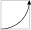
\includegraphics[width=0.5cm]{rasdemo}
    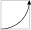
\includegraphics[width=1cm]{rasdemo}
    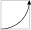
\includegraphics[width=2cm]{rasdemo}
    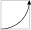
\includegraphics[width=4cm]{rasdemo}\\
    Raster
  \end{minipage}
  \begin{minipage}{0.4\linewidth}
    \centering
    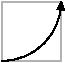
\includegraphics[width=0.5cm]{vecdemo}
    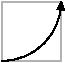
\includegraphics[width=1cm]{vecdemo}
    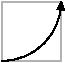
\includegraphics[width=2cm]{vecdemo}
    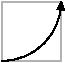
\includegraphics[width=4cm]{vecdemo}\\
    Vector
  \end{minipage}
  \caption{Difference between raster and vector graphics}
  \label{fig:rastervector}
\end{figure}

Most of the graphics in an engineering report will be represented well
using vector graphics.  They work well for plots, graphs and line
drawings of equipment.  They result in small file sizes and produce
high quality output when printed.  Examples of file extensions for
vector files are SVG, EPS, WMF, EMF and Visio files.  Raster graphics will
probably be used exclusively for photographs or screen captures of
computer software.  Examples of file extensions for raster files are
BMP, PNG, GIF, TIFF, and JPG.

When preparing screen captures, another important aspect of the
graphic file format is the type of compression used.  Most common
raster file formats are \emph{lossless}, retaining all of the
information in the original file.  The JPG file format, however, was
designed to compress photographs and uses \emph{lossy} compression
based on mathematical reduction of the information in the original
file.  The effect of this compression can be seen in
Figure~\ref{fig:jpgexample}, where a screenshot was taken and saved as
a PNG file and a JPG file.

\begin{figure}[htbp]
  \centering
  
\includegraphics[width=\textwidth]{screenshot_lossless}
  
\includegraphics[width=\textwidth]{screenshot_lossy}
  \caption{Lossless compression (PNG) vs lossy compression (JPG).
    Note the noise or ``artifacts'' in the second image}
  \label{fig:jpgexample}
\end{figure}

The routines used to compress the image in JPG are optimised for
photographs and should only be used for images with ``natural''
characteristics, rather than computer generated images.

Most students will incorporate graphics into a word-processor using
``copy and paste''.  This may cause the format of the file to be
unknown.  It is recommended that all graphics be saved as separate
files and then inserted into the document.  This will not only ensure
that the document retains a manageable size, but will make it easier
to exchange graphics as well.

\subsection{Equations}
\label{sec:tips-equations}
To insert an equation according to our guidelines in Word 2003 you can
follow these steps:
\begin{enumerate}
\item Insert a 1$\times$3 table in Word, and make the column width of
  column 1 and 3 15\%.
\item Next insert an equation in the middle column. Don't enter an
  equation.
\item Place the cursor to the right of the equation in the middle
  column.
\item Go to References | Insert Caption in the menu. Select
  ``Equation'' next to label and select the ``Exclude label from
  caption'' checkbox. See figure~\ref{fig:wordcaption}
\item Move the caption to the third column and surround it in
  parentheses.
\item Remove the borders from the table
\item Select the whole table
\item Save the equation to the gallery by selecting
  ``Insert|Equation|Save Selection to Equation Gallery.
\end{enumerate}
\begin{figure}[htbp]
  \centering
  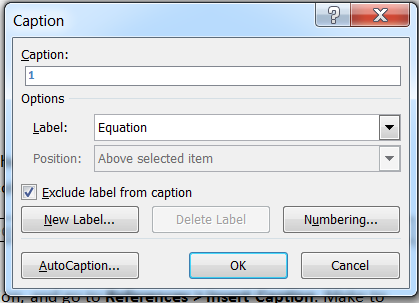
\includegraphics[width=0.5\textwidth]{captionwindow}
  \caption{The Insert Caption window in Word 2003}
  \label{fig:wordcaption}
\end{figure}
Now you can insert this equation into a document using this building
block.  You can cross-reference this equation by going to
``References|Cross reference'' and selecting the ``Equation''
reference type.  You will see the window shown in
figure~\ref{fig:wordcrossref}.  You can then select the equation from
the list.  It will be kept up to date automatically.
\begin{figure}[htbp]
  \centering
  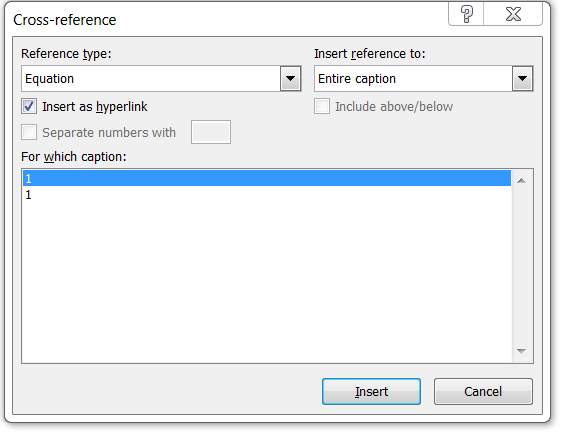
\includegraphics[width=0.7\textwidth]{crossreference}
  \caption{The Cross-reference window in Word 2003}
  \label{fig:wordcrossref}
\end{figure}

\subsection{Special characters}
There are a number of special characters which are commonly mistyped
or incorrectly entered.  Never resort to using a different font like
Symbol to enter your special symbols.  Rather use the Unicode code
point for the character you are looking for.
Table~\ref{tab:specialchar} shows a number of common symbols.  On MS
Windows, these characters can be entered by holding the Alt key and
then entering the code point including the leading zero.  For example,
to enter the multiplication sign, press and hold Alt while entering
00D7, then let go of the Alt key.
\begin{table}[htbp]
  \centering
  \caption{Unicode code points for commonly used special characters}
  \label{tab:specialchar}
  \begin{tabular}{lcll}
    \toprule
    Name                                                                                                  & Symbol               & Code point & Name                \\ 
    \midrule
    Degree                                                                                                & \SI{}{\degree}       & U+00B0     & degree sign         \\ 
    Multiplication                                                                                        & $\times$             & U+00D7     & multiplication sign \\
    Chemical equilibrium                                                                                  & $\rightleftharpoons$ & U+021CC    & rightleftharpoons   \\
    \AA ngstr\"om                                                                                         & \SI{}{\angstrom}     & U+212B     & angstrom sign       \\
    Multiplication dot                                                                                    & $\cdot$              & U+22C5     & dot operator        \\
    \bottomrule
  \end{tabular}
\end{table}
% TODO: consider all the stuff in this table
% https://publications.csiro.au/rpr/download?pid=csiro:EP115755 &
% dsid=DS4

\subsection{Formatting}
\label{sec:tips-formatting}
There are often problems with line breaks when certain words need to
be kept together.  A common example is a number and its unit or the
number \num{1.2e4}.  It is bad form for such elements to be broken at
the end of a line.  The solution to this problem is the
\emph{non-breaking space}.  In Microsoft Word, a non-breaking space is
inserted by pressing Ctrl-Shift-Space.  In \LaTeX, use \verb|~|.

% FIXME \textbf{I need advice from Word users on correct ways of
% including figures, tables, references and cross-references}

% \subsection{Figures and tables}

% \subsection{References}

% \subsection{Cross-references}

% \section{Gallery}
% \label{cha:gallery}
% This chapter contains examples of good and bad practise.  Use it to
% identify problems in your reports and find out how to fix them.

% \section{Useful links}
% The NIST Reference on Constants, Units, and Uncertainty
% \url{http://physics.nist.gov/cuu/}
%

% \section{Grammatical errors}
% \label{app:grammatical-errors}

% Some common grammatical errors should be avoided assiduously:

% \begin{description}
% \item[Split infinitives] The infinitive form of a verb is the
%   structure ``to \emph{verb}''.  These two words should be seen as a
%   unit and should not be split with adverbs as in ``to easily do''.
%   Rather use ``to do easily''.  See
%   \url{http://en.wikipedia.org/wiki/Split_infinitive}.
% \item[Dangling participle] Ensure that modifiers (especially
%   participles) attach clearly to the words they are modifying.  A
%   common example of incorrect usage is ``Substituting Equation 1
%   into Equation 2 gives \dots''.  The following two examples are
%   gramatically sound: ``Substitution of Equation 1 into Equation 2
%   gives \dots'' and ``By substituting Equation 1 in Equation 2, we
%   obtain \dots''.
%   See~\url{http://en.wikipedia.org/wiki/Dangling_modifier}.
% \end{description}

\end{document}